% === Begin Label Data ===
% ID: 441
% 难度星级: 
% 标签: 
% 备注: 
% 组卷引用次数: 0
% === End  Label Data ===

\begin{problem}{1990}{G}{全国卷}{11}{立体几何}
如图，正三棱锥 $ S-ABC $ 的侧棱与底面边长相等，如果 $ E $、$ F $ 分别为 $ SC $、$ AB $ 的中点，那么异面直线 $ EF $ 与 $ SA $ 所成的角等于 (\hspace{1cm})
\begin{choices}
\choice{{$90^\circ$}}
\choice{{$60^\circ$}}
\choice{{$45^\circ$}}
\choice{{$30^\circ$}}
\end{choices}
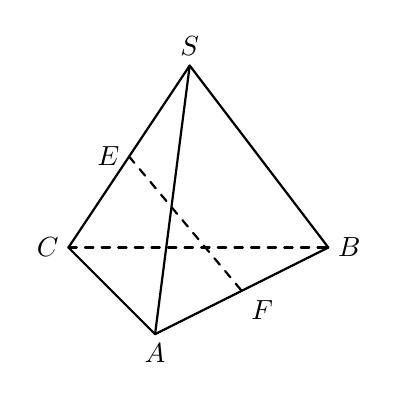
\begin{tikzpicture}[scale=1.1, line cap=round, line join=round]
\usetikzlibrary{calc}
\coordinate (A) at (0,0);
\coordinate (B) at (2,1);
\coordinate (C) at (-1.0,1.0);
\coordinate (S) at (0.4,3.1);

\coordinate (E) at ($(S)!0.5!(C)$);
\coordinate (F) at ($(A)!0.5!(B)$);

\draw[thick] (S)--(A);
\draw[thick] (S)--(B);
\draw[thick] (S)--(C);

\draw[thick] (A)--(B);
\draw[thick] (A)--(C);
\draw[dashed,thick] (C)--(B);

\draw[dashed,thick] (E)--(F);

\node[below] at (A) {$A$};
\node[right] at (B) {$B$};
\node[left]  at (C) {$C$};
\node[above] at (S) {$S$};
\node[left]  at (E) {$E$};
\node[below right] at (F) {$F$};
\end{tikzpicture}
\end{problem}

\begin{answer}

\end{answer}

\begin{solutions}

\end{solutions}